\chapter*{付録} % 章番号を出さない
\addcontentsline{toc}{chapter}{付録} % 目次に載せる

「付録」(appendix)は、論文の本文に載せるには情報として邪魔もしくは必須ではないものの、読者にとって有益となるような情報を載せます。付録を必要としない論文ももちろん存在しますので、そこは著者の判断です。

例えば、たくさんの観測データを様々なモデルでフィットした場合、フィット結果の絵がたくさん出てくるはずです。そのような図は本文中に大量に出されても大切な情報を見失ってしまいますので、大部分は付録に載せることが推奨されます。他には、何かしらの長い式変形や証明を載せる必要がある場合、付録に移動する場合があります。

% 付録は chapter の 1 つとして作りますが、章番号は表示しません。
% また付録の 1 つずつはアルファベットで番号付けをするのが一般的です。
\setcounter{section}{0} % section の番号をゼロにリセットする
\renewcommand{\thesection}{\Alph{section}} % 数字ではなくアルファベットで数える
\setcounter{equation}{0} % 式番号を A.1 のようにする
\renewcommand{\theequation}{\Alph{section}.\arabic{equation}}
\setcounter{figure}{0} % 図番号
\renewcommand{\thefigure}{\Alph{section}.\arabic{figure}}
\setcounter{table}{0} % 表番号
\renewcommand{\thetable}{\Alph{section}.\arabic{table}}

\section{すごい長い証明}
式~(\ref{eq})のように、式番号がアルファベットとアラビア数字の組み合わせになるように、\LaTeX{}ソース中で設定してありますので、中身を眺めてみてください。

\begin{equation}
  \label{eq}
  1 + 1 = 2
\end{equation}


\section{すごいたくさんのフィットの図}

\section{修士論文添削前に自己点検する項目}

\begin{itemize}
\item[\CID{00728}] 第\ref{chap:plagiarism}章を読み、剽窃について十分に理解したか。
\item[\CID{00728}] 修士論文に剽窃箇所もしくは剽窃と見なされうる箇所は存在しないか。
\item[\CID{00728}] \LaTeX\ で図番号などの参照先がないせいで「図??」「表??」「??節」のようになっている箇所はないか。
\item[\CID{00728}] 日本語読点「、」と欧文カンマ「,」が混在していないか。例えば「ガンマ線望遠鏡は、HESS, MAGIC, VERITASなどがある」。
\item[\CID{00728}] 日本語丸括弧「()」と欧文丸括弧「()」が混在していないか。
\item[\CID{00728}] 単位と数値の間にスペースは入っているか。「100MeV」など。
\item[\CID{00728}] 単位が斜体になっていないか。「$100~MeV$」など。
\item[\CID{00728}] 変数でない添字などが斜体になっていないか。$N_{trigger}$など。
\item[\CID{00728}] 自分で作成したものではない図や写真は、全て出典が明記され、転載であることを書いてあるか。
\end{itemize}

\section{無限運動量飛跡試験に際して行われた修正}
\label{sec:appendix:infinite-momentum-tracks}
無限運動量飛跡の試験で明らかになったトリガー回路の修正点とそのデバッグの過程について述べる。図\ref{}に修正を行う前の結果を示す。トリガー回路のデバッグ前の段階では多くのInefficiencyが見られた。\ref{}章で述べたようにトリガー回路はこれまでにソフトウェアシミュレーターとVivado シミュレーターで動作検証は行われてきたが、これらのInefficiencyは大統計量を用いた網羅的な試験によって初めて発見されたものである。以下にそれぞれのモジュールにおけるInefficiencyとその解決について述べる。

\begin{figure}
  \begin{minipage}[b]{.5\linewidth}
      \centering
      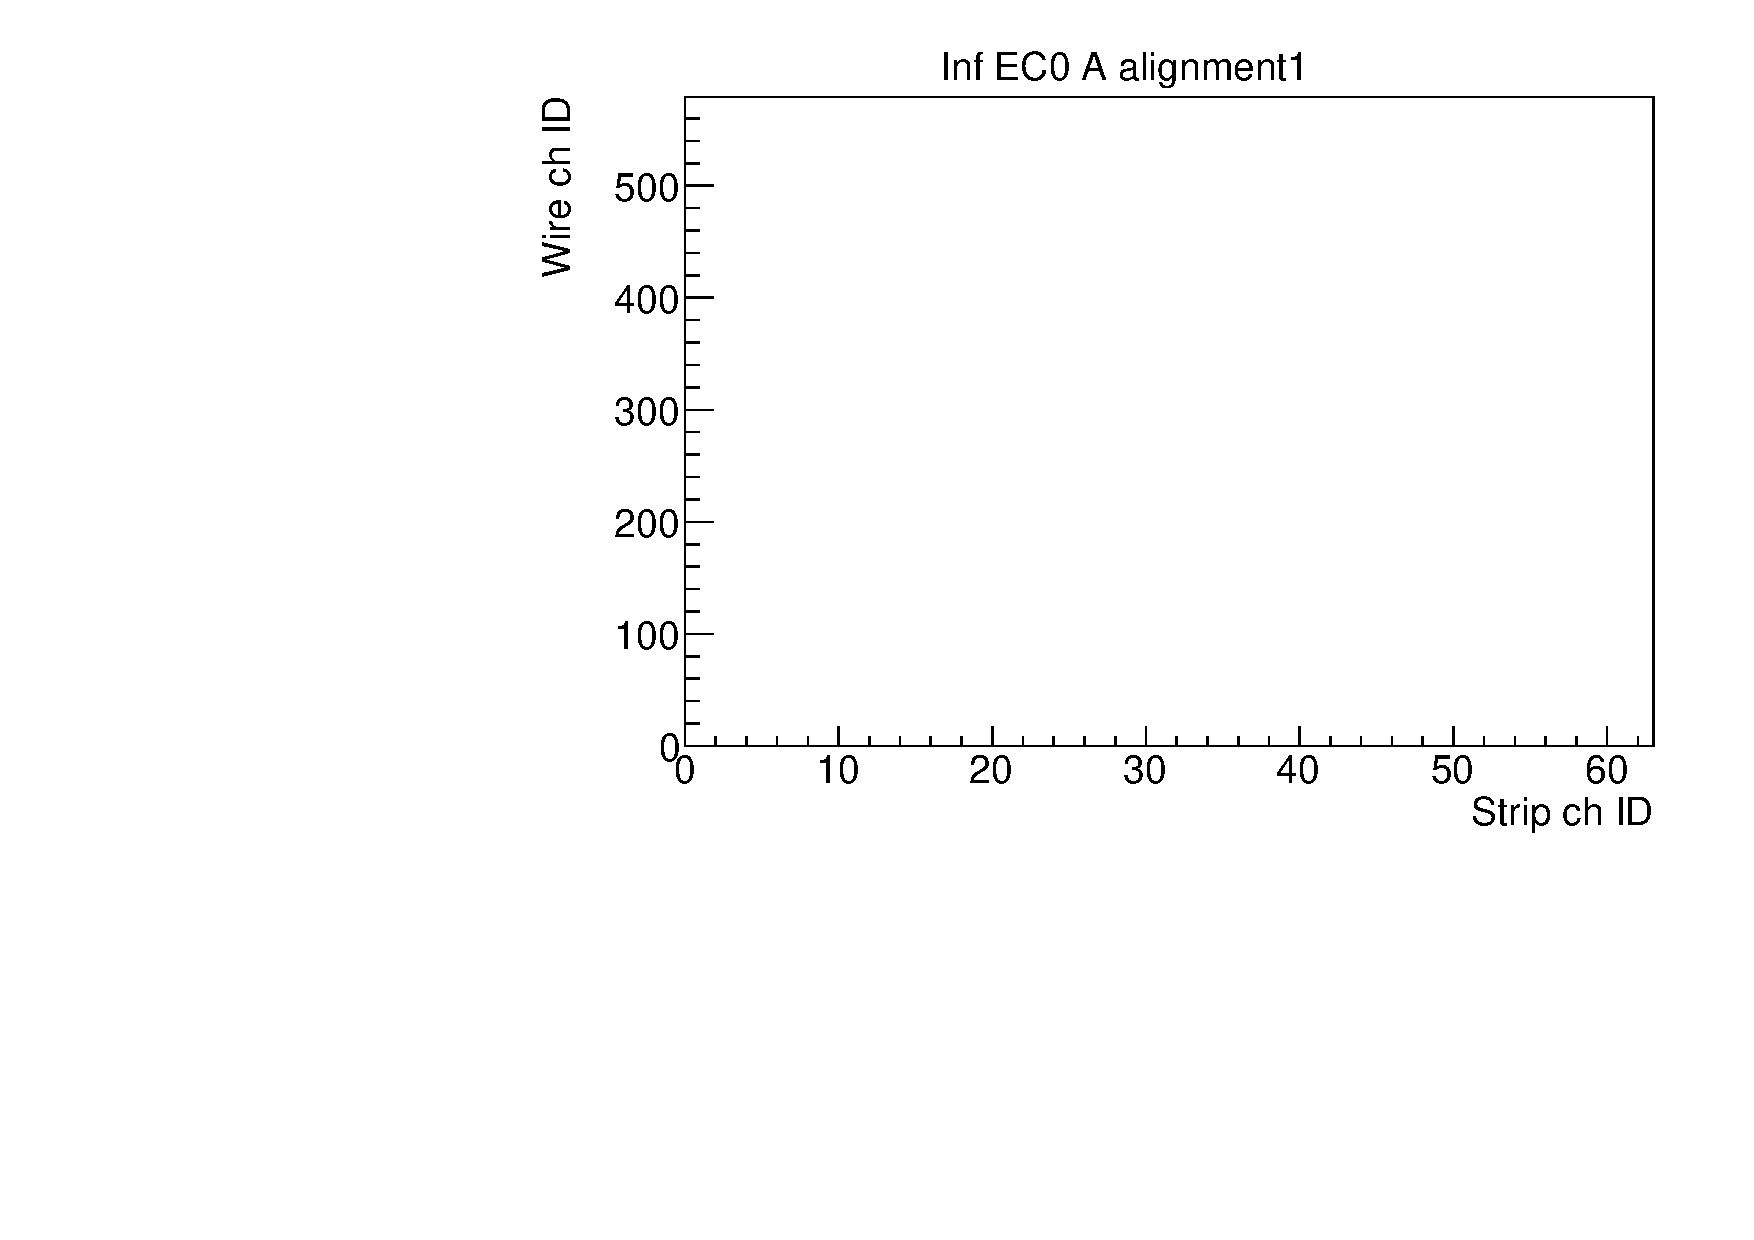
\includegraphics[height=6cm]{fig/Test/B_InfEC0_strip.pdf}
      \subcaption{エンドキャップ$\phi\,$0領域の結果}
  \end{minipage}
  \begin{minipage}[b]{.5\linewidth}
      \centering
      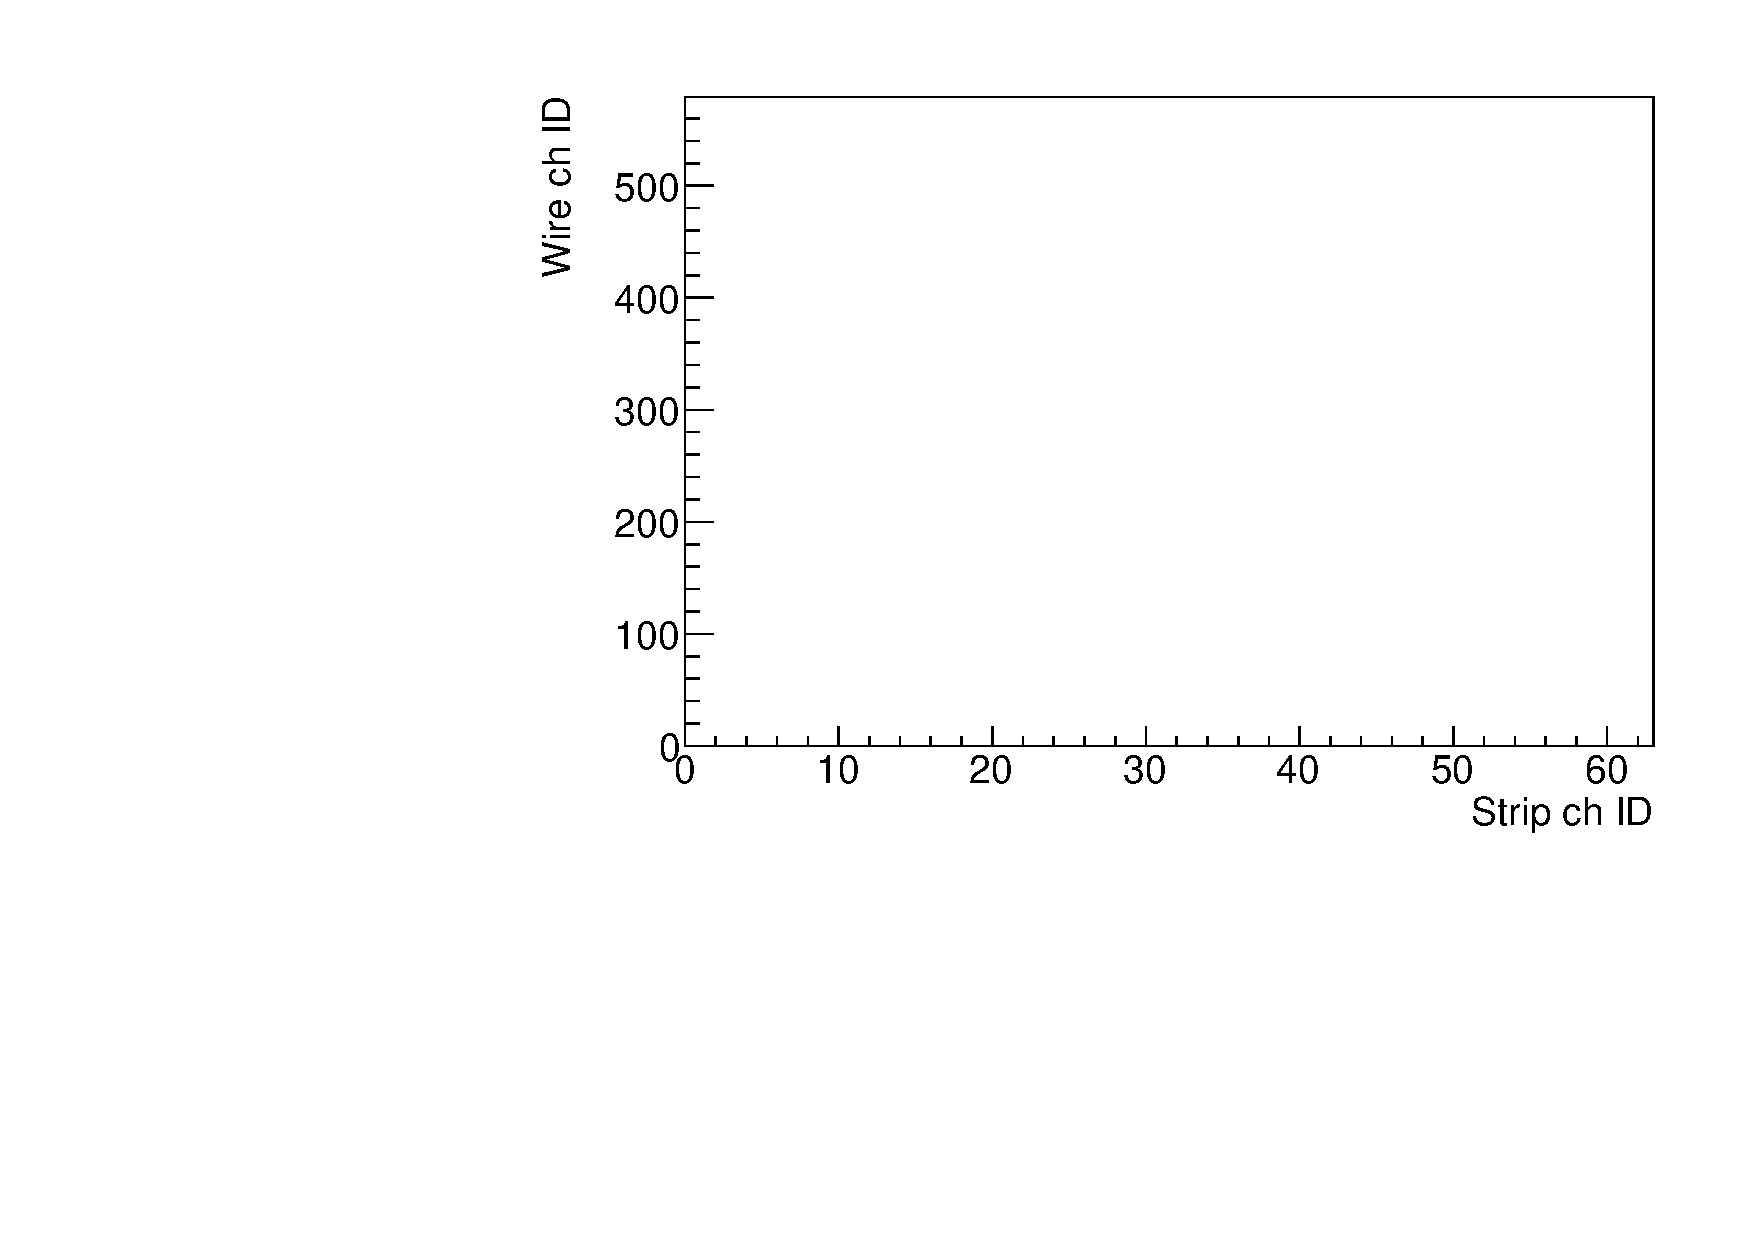
\includegraphics[height=6cm]{fig/Test/B_InfEC1_strip.pdf}
      \subcaption{エンドキャップ$\phi\,$1領域の結果}
  \end{minipage}\\
  \begin{minipage}[b]{\linewidth}
      \centering
      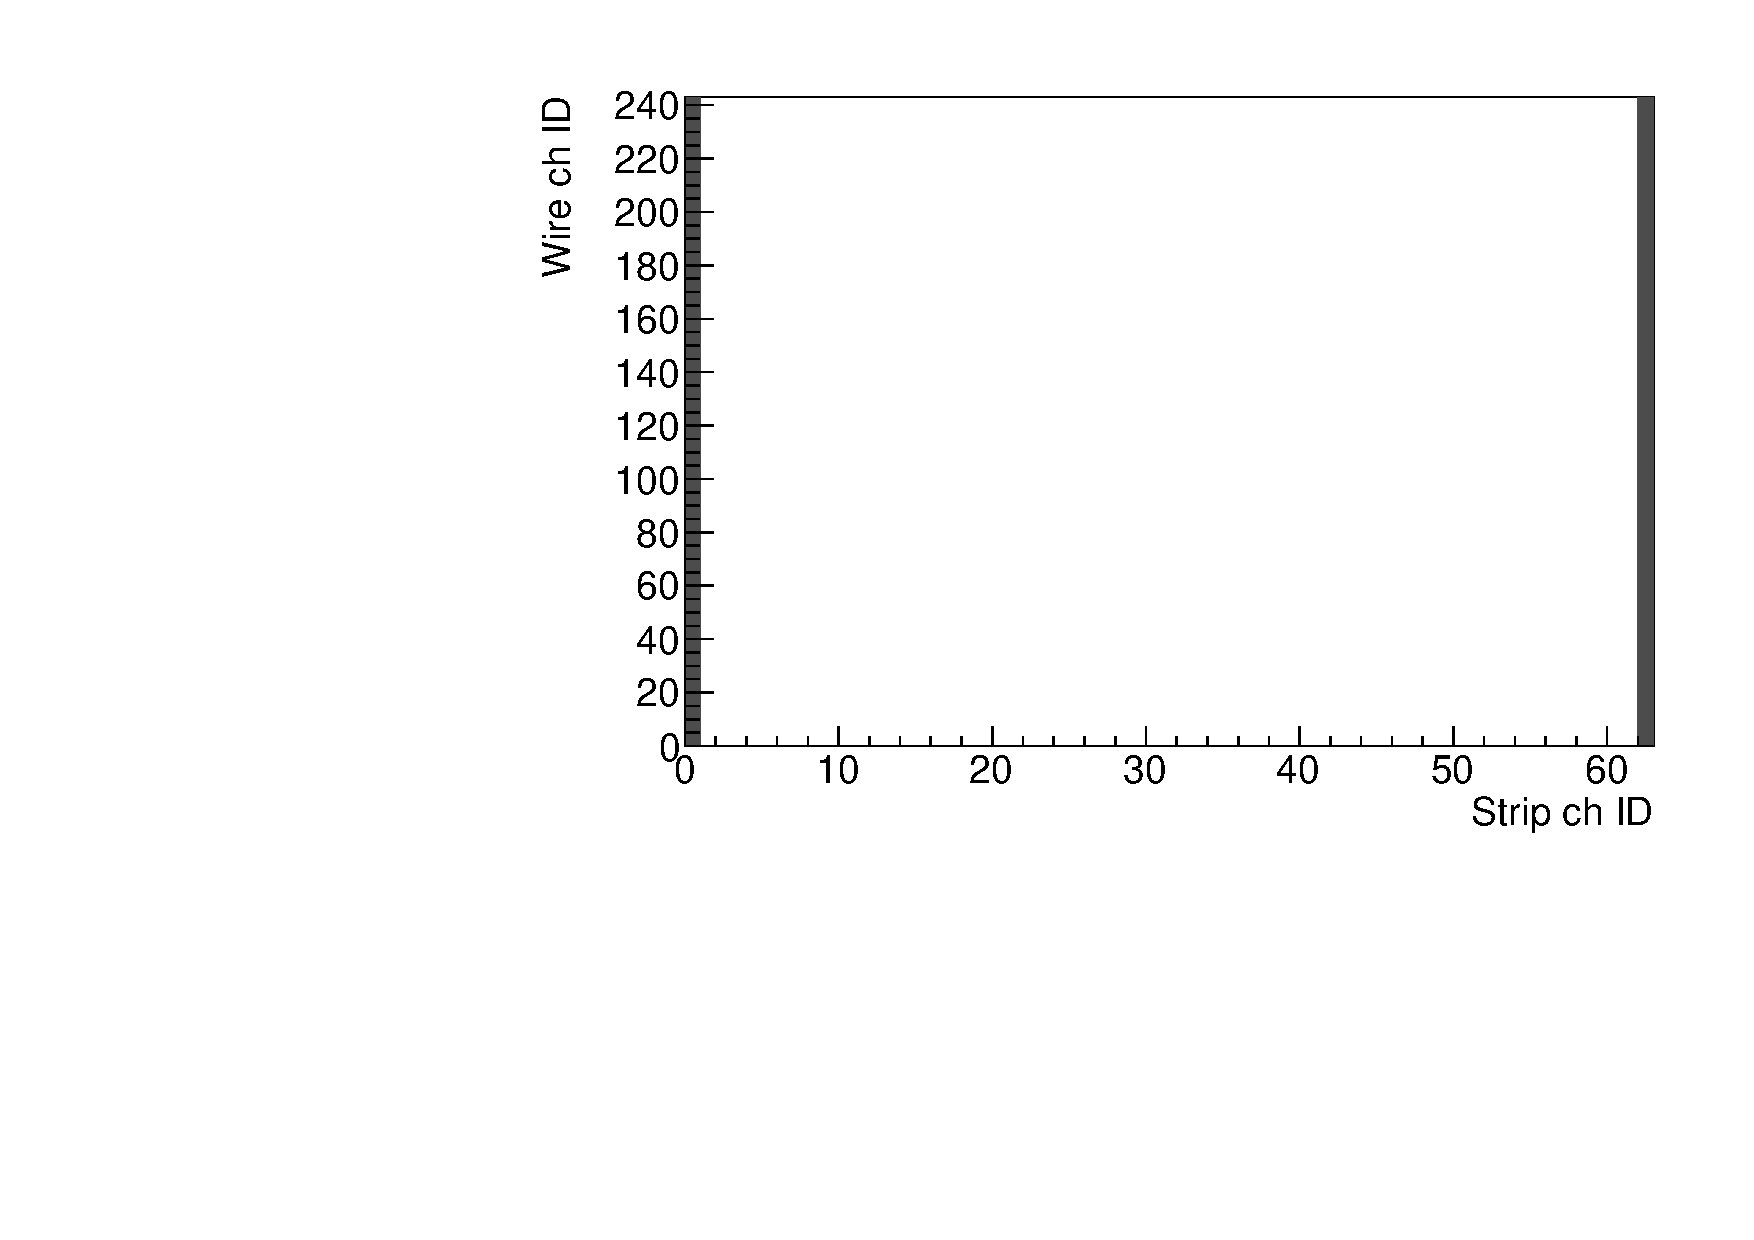
\includegraphics[height=6cm]{fig/Test/B_InfFW_strip.pdf}
      \subcaption{フォワード領域の結果}
  \end{minipage}
  \caption[異なる画像形式の比較]{無限運動量飛跡に対する、Strip Segment Reconstructionの応答。}
  \label{Inf_B_Strip}
  \end{figure}
  
  \begin{figure}
      \begin{minipage}[b]{.5\linewidth}
          \centering
          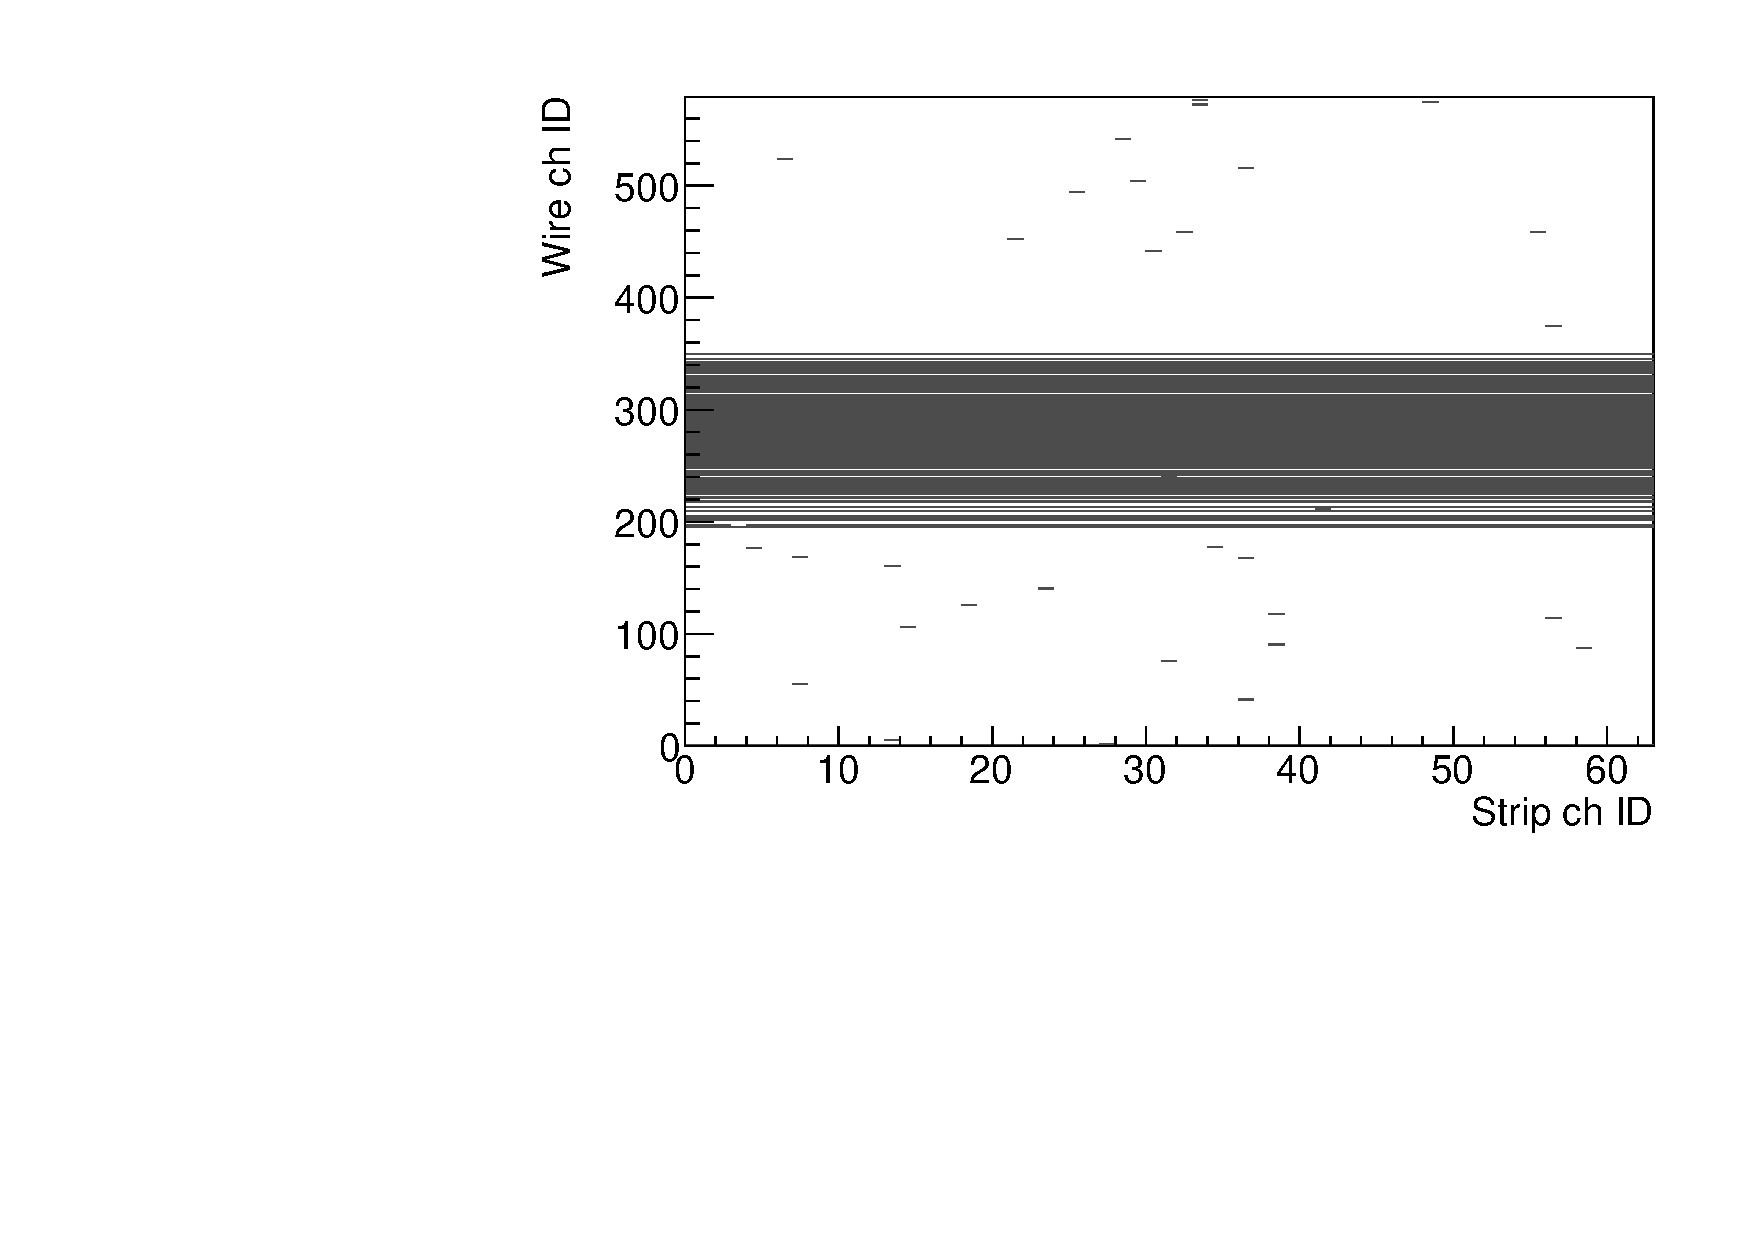
\includegraphics[height=6cm]{fig/Test/B_InfEC0_wire.pdf}
          \subcaption{エンドキャップ$\phi\,$0領域の結果}
      \end{minipage}
      \begin{minipage}[b]{.5\linewidth}
          \centering
          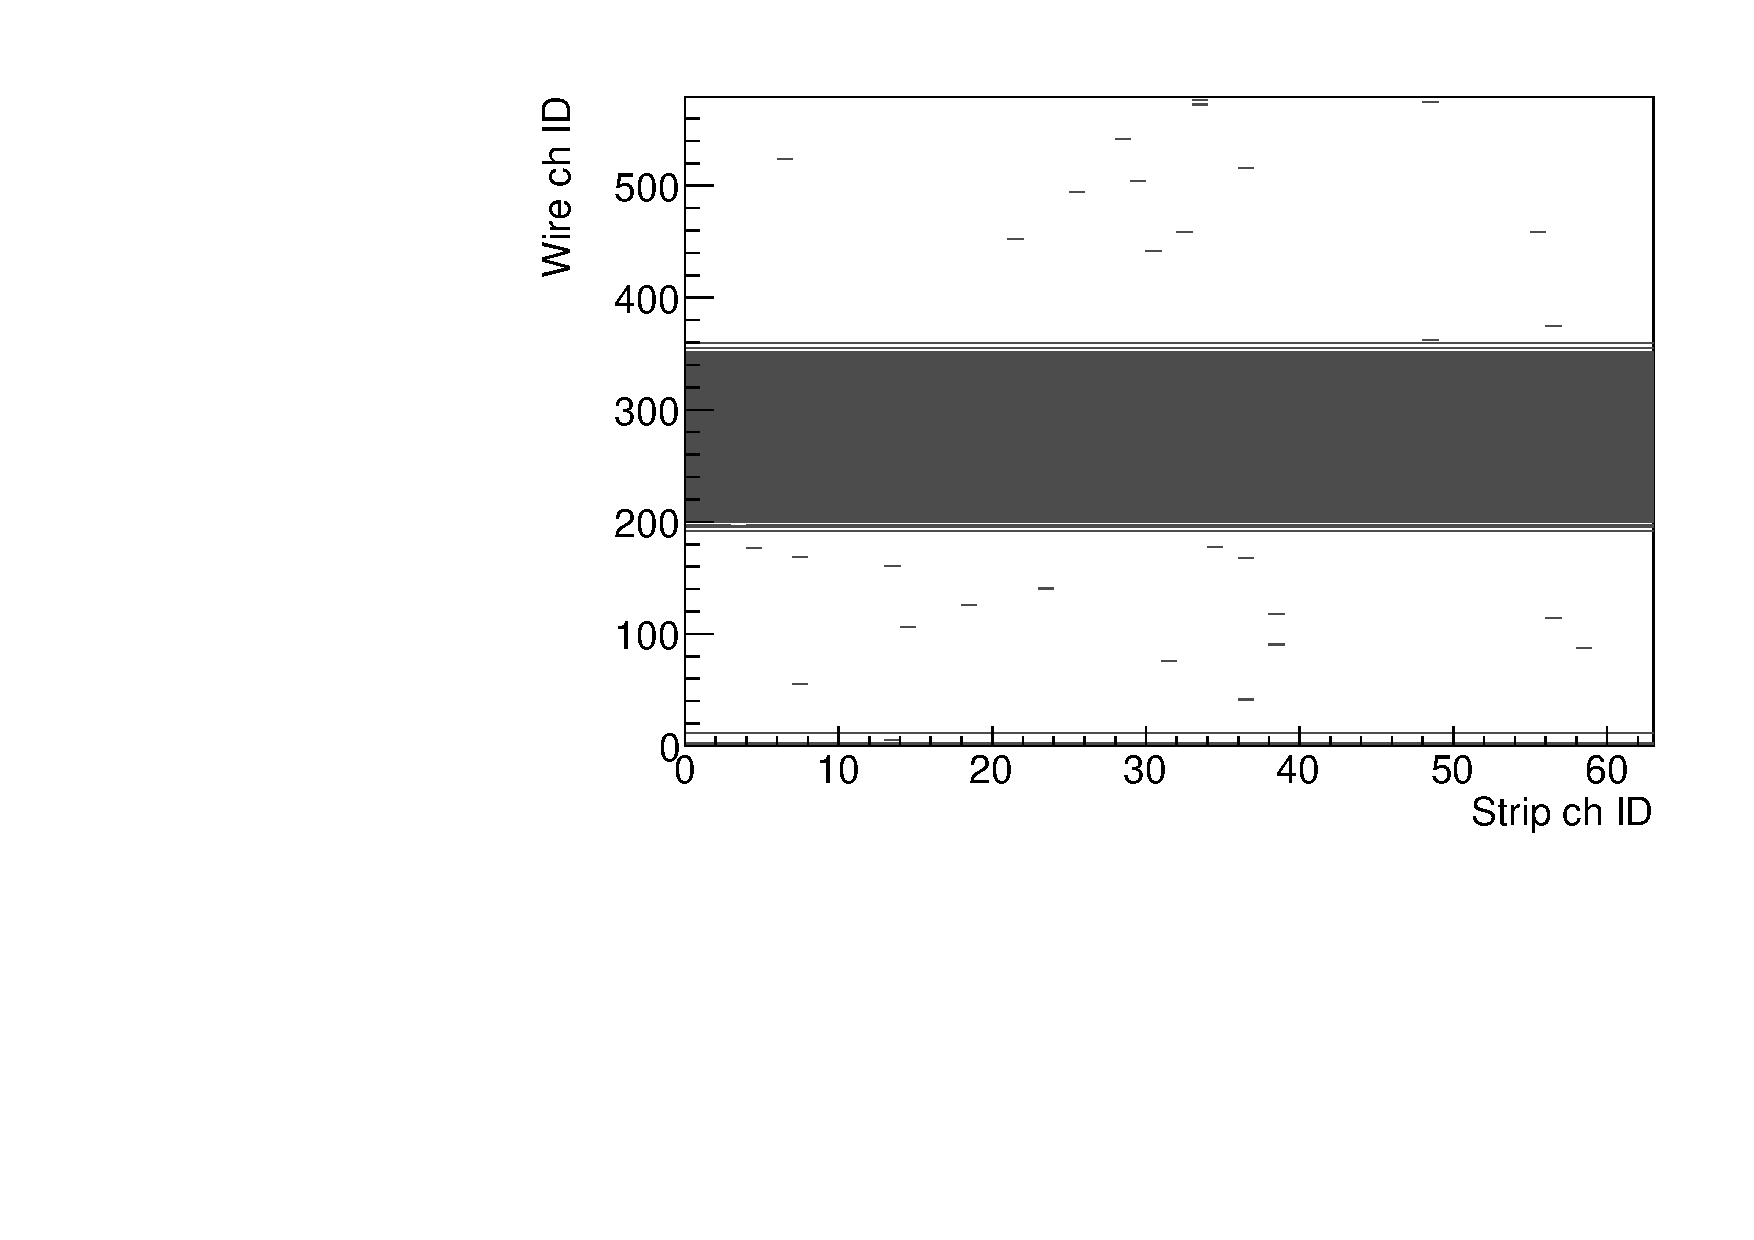
\includegraphics[height=6cm]{fig/Test/B_InfEC1_wire.pdf}
          \subcaption{エンドキャップ$\phi\,$1領域の結果}
      \end{minipage}\\
      \begin{minipage}[b]{\linewidth}
          \centering
          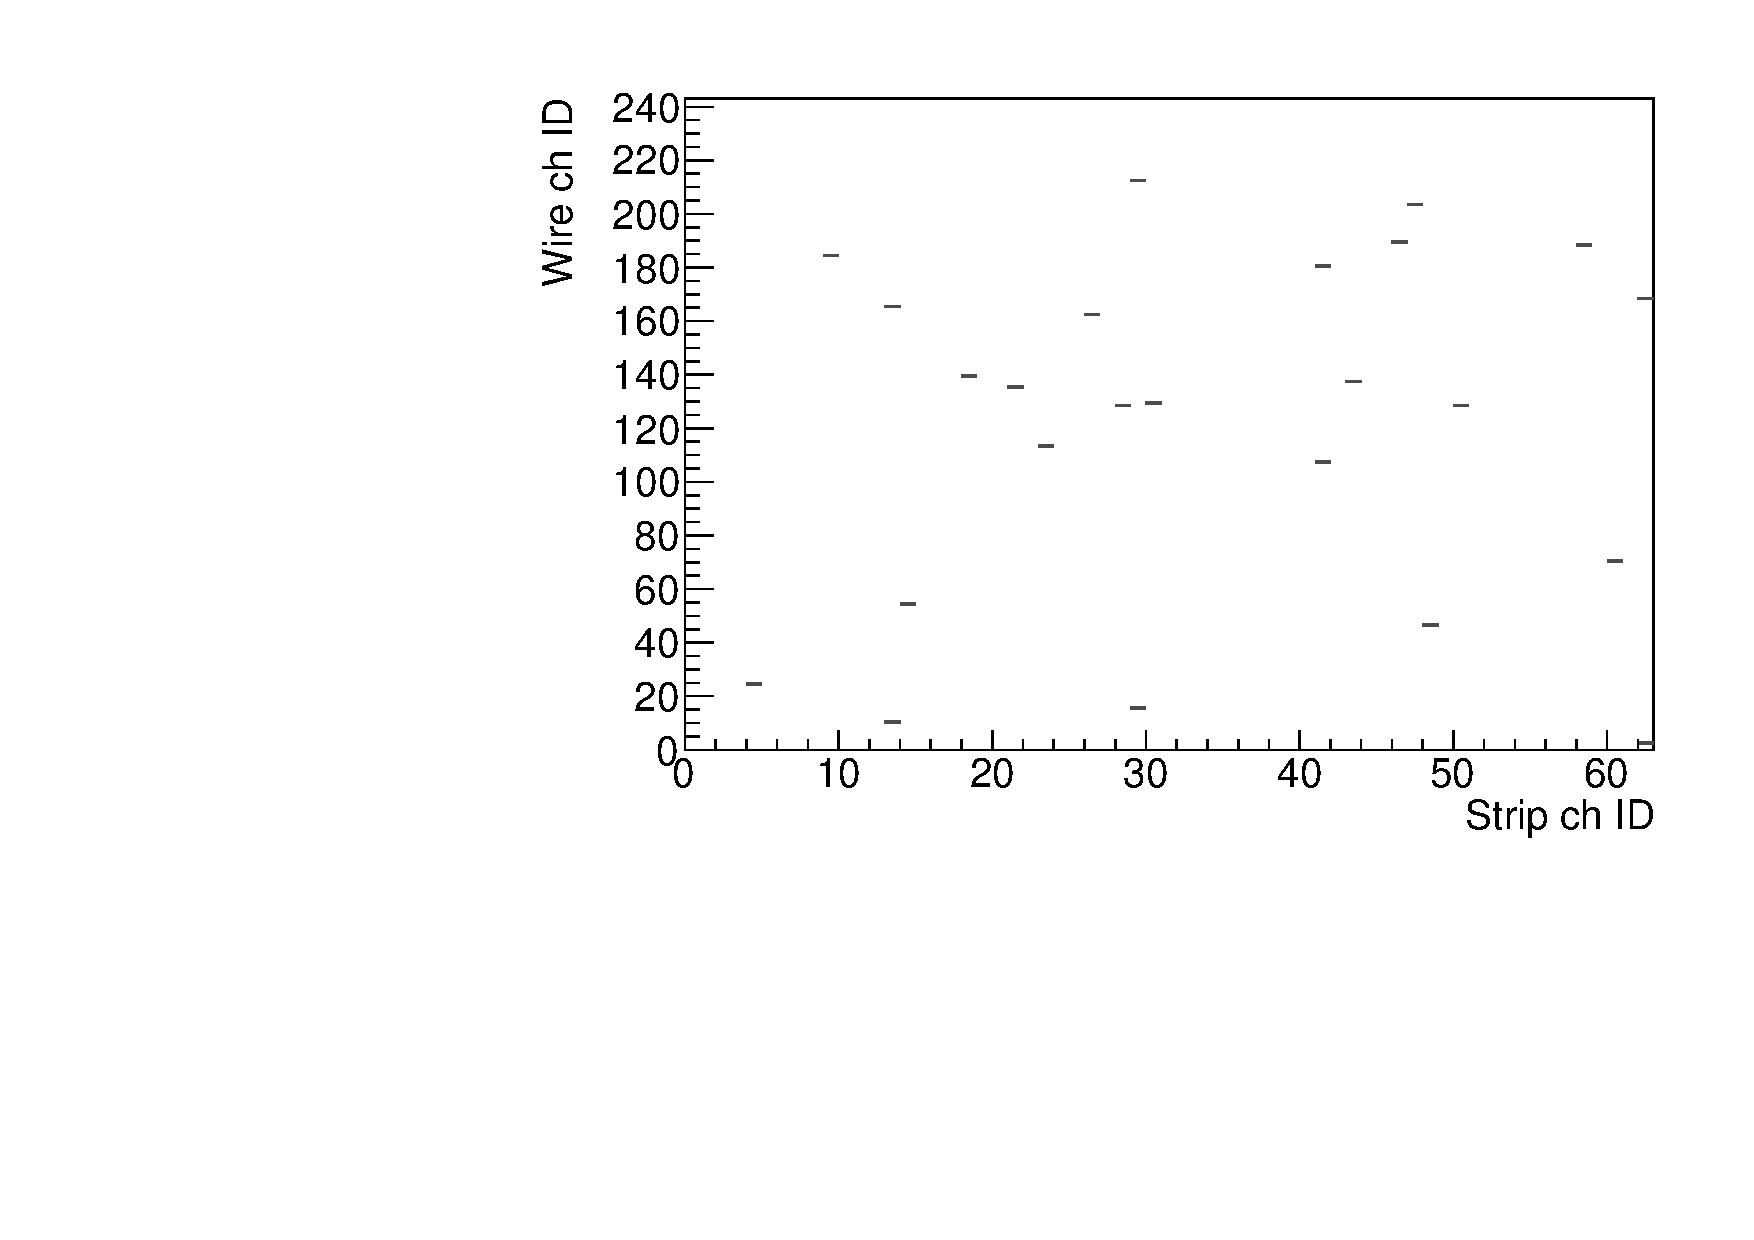
\includegraphics[height=6cm]{fig/Test/B_InfFW_wire.pdf}
          \subcaption{フォワード領域の結果}
      \end{minipage}
      \caption[異なる画像形式の比較]{無限運動量飛跡に対する、Wire Segment Reconstructionの応答。}
      \label{Inf_B_Wire}
  \end{figure}
  
  \begin{figure}
      \begin{minipage}[b]{.5\linewidth}
          \centering
          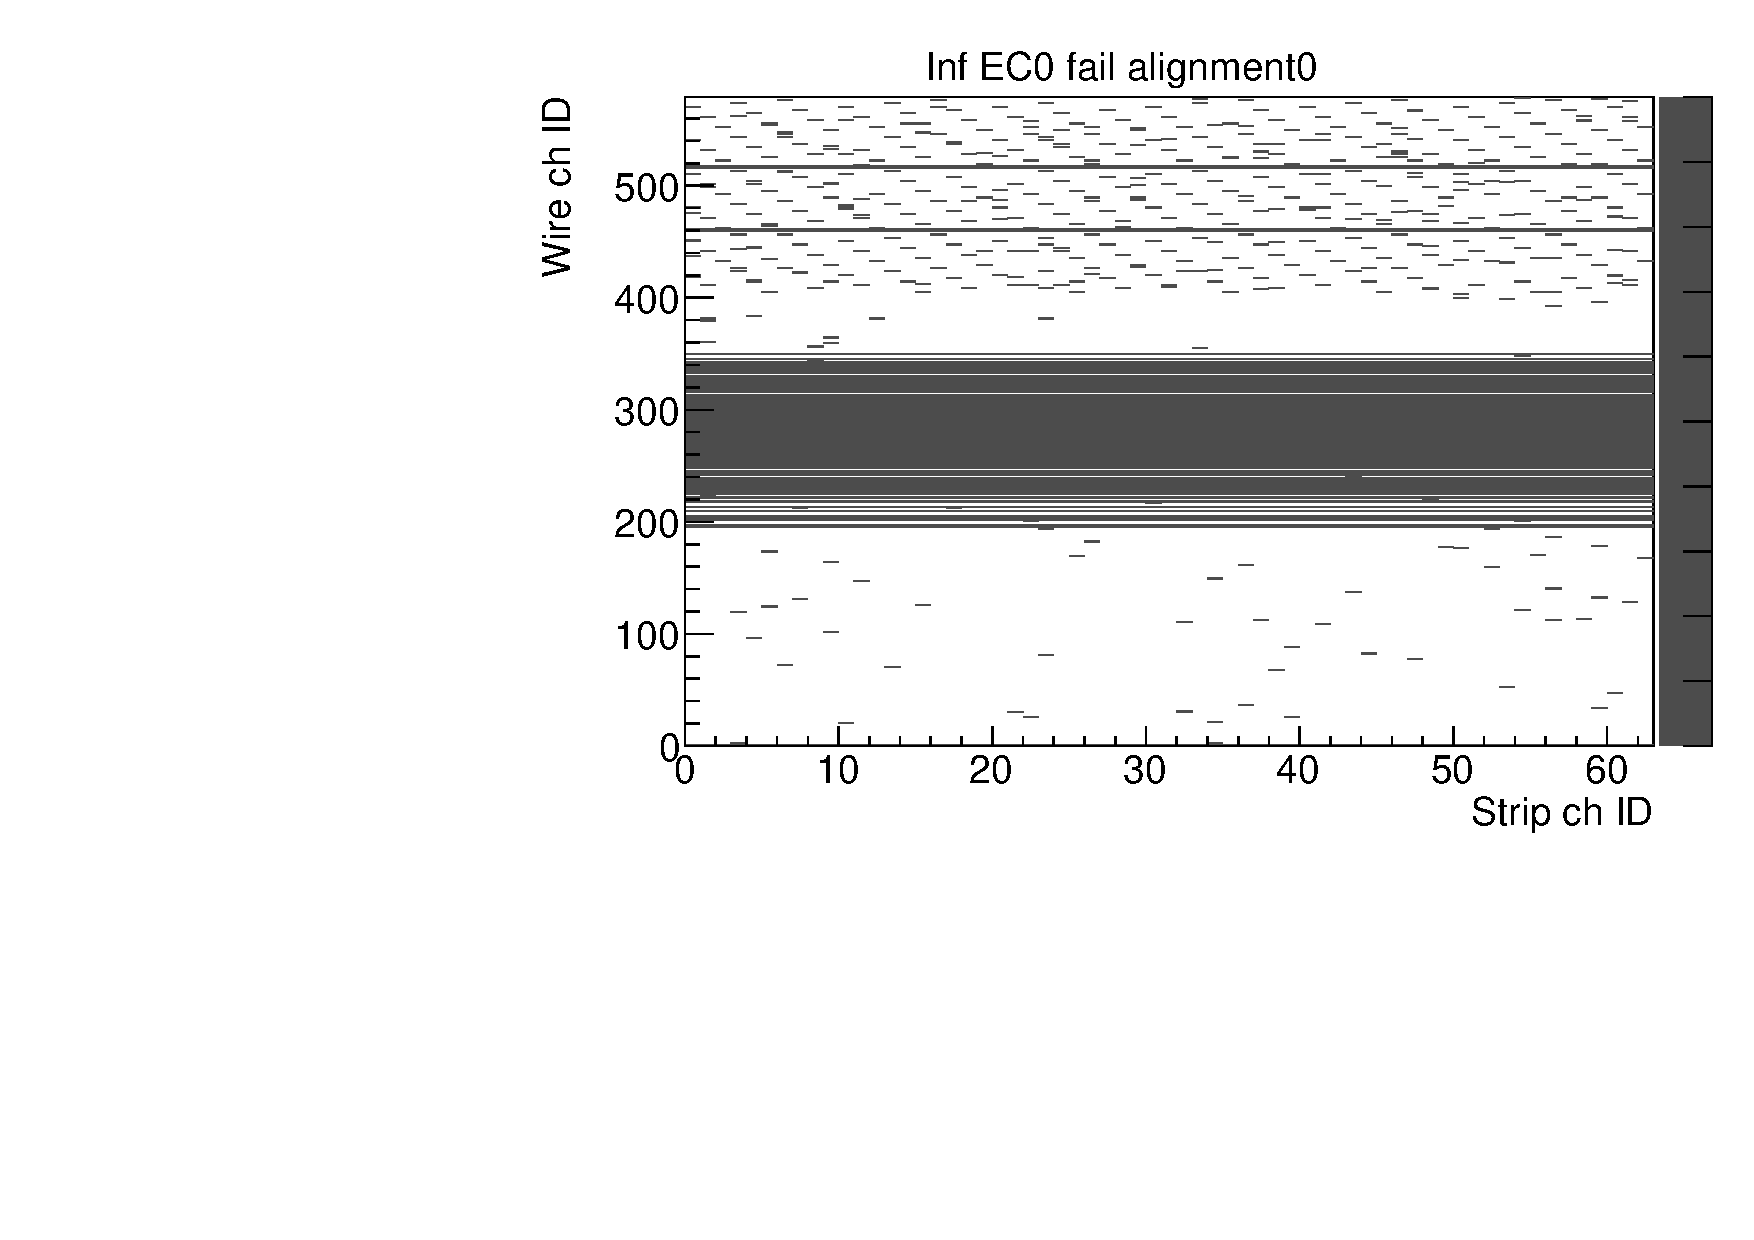
\includegraphics[height=6cm]{fig/Test/B_InfEC0_WS.pdf}
          \subcaption{エンドキャップ$\phi\,$0領域の結果}
      \end{minipage}
      \begin{minipage}[b]{.5\linewidth}
          \centering
          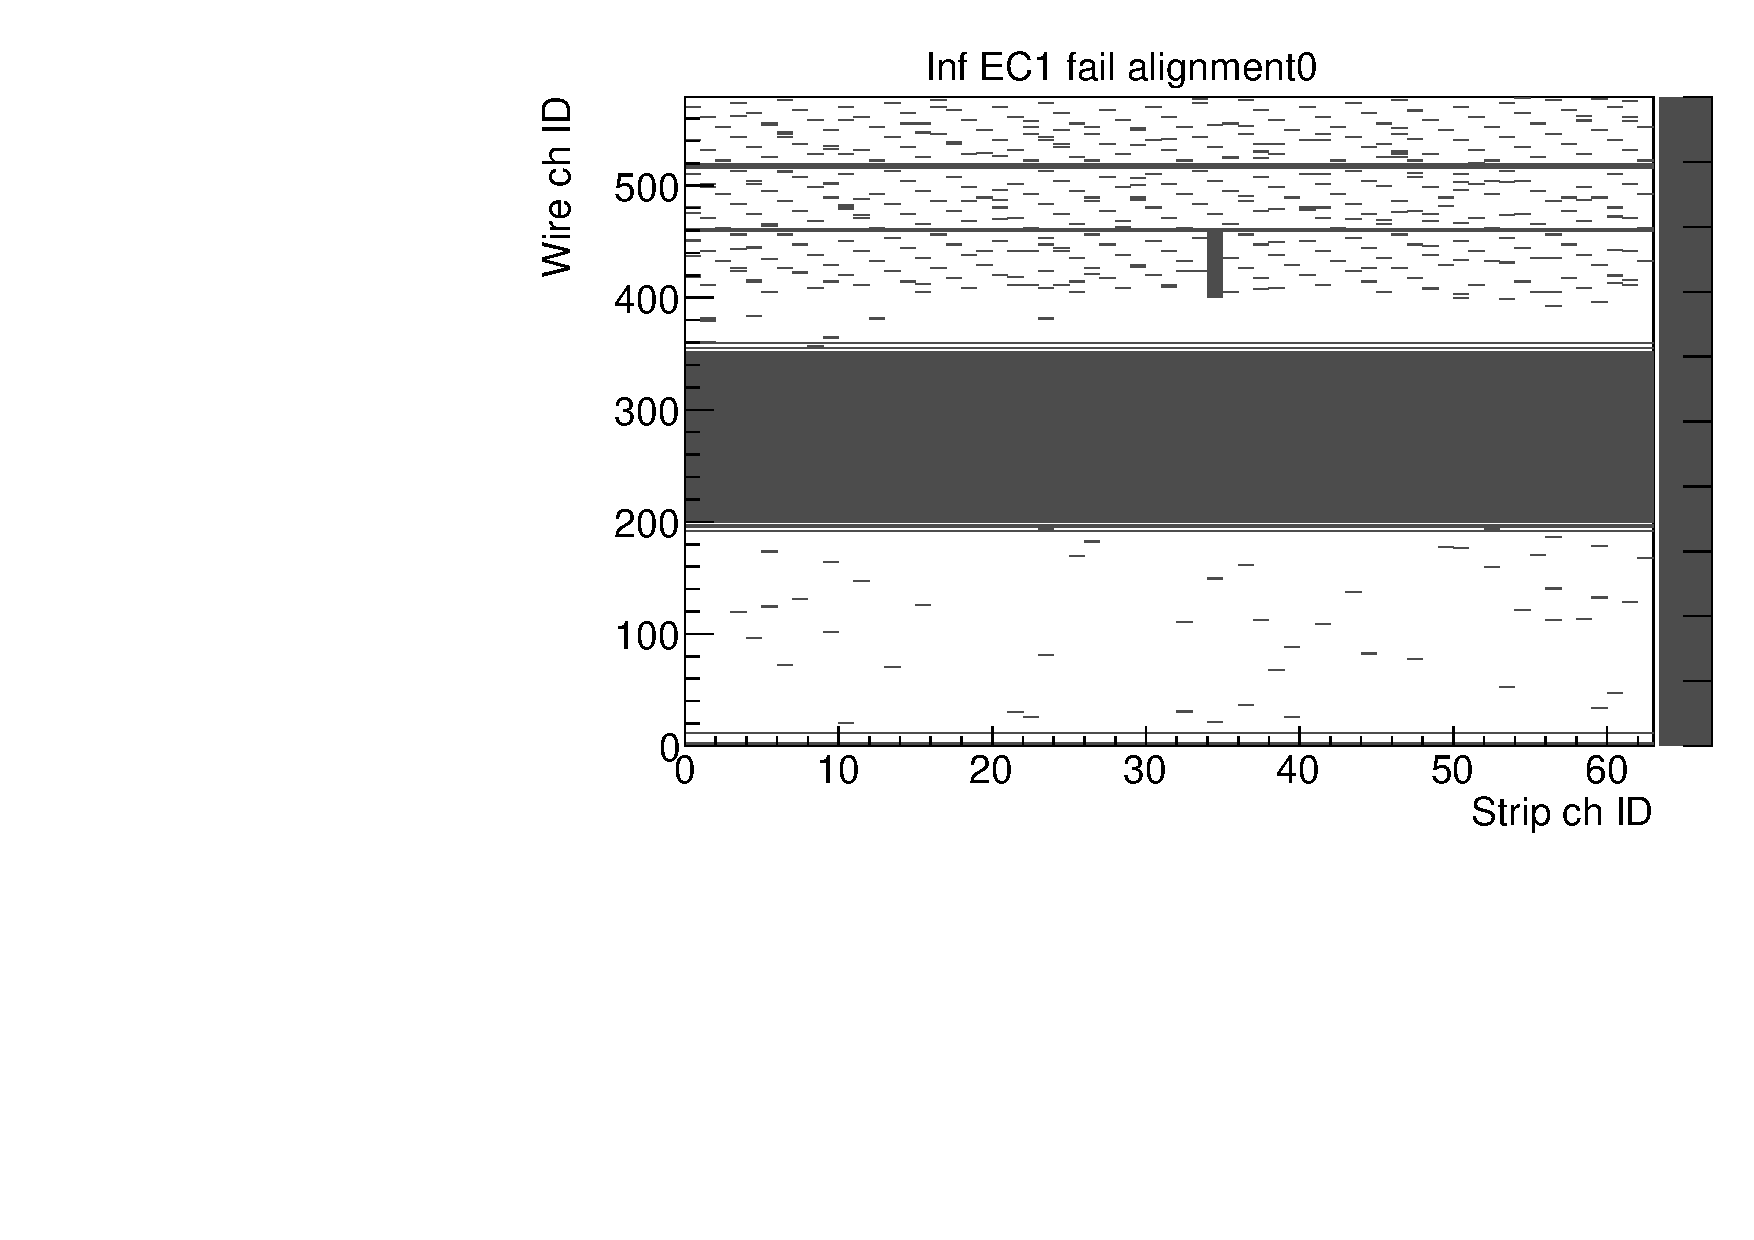
\includegraphics[height=6cm]{fig/Test/B_InfEC1_WS.pdf}
          \subcaption{エンドキャップ$\phi\,$1領域の結果}
      \end{minipage}\\
      \begin{minipage}[b]{\linewidth}
          \centering
          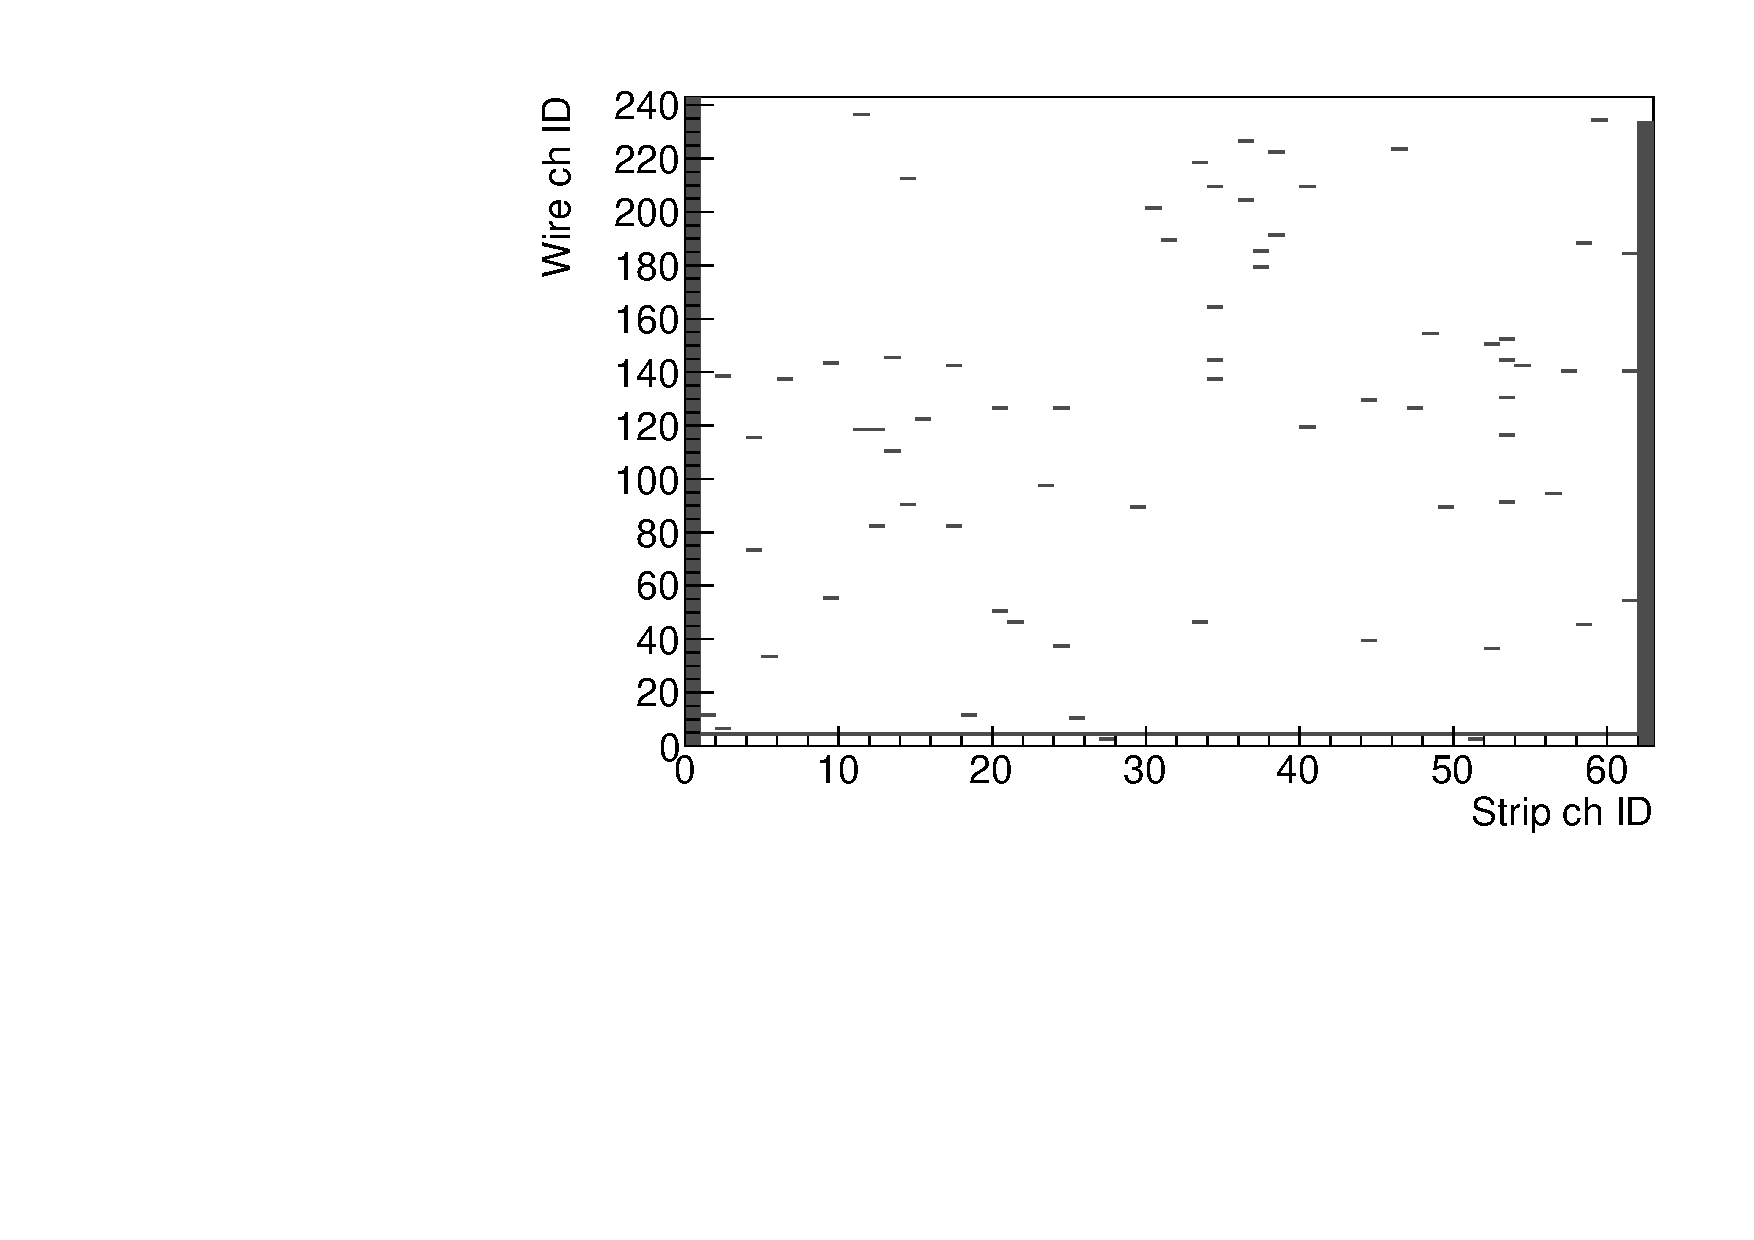
\includegraphics[height=6cm]{fig/Test/B_InfFW_WS.pdf}
          \subcaption{フォワード領域の結果}
      \end{minipage}
      \caption[異なる画像形式の比較]{無限運動量飛跡に対する、Wire Strip Coincidenceの応答。}
      \label{Inf_B_WS}
  \end{figure}

\paragraph{Strip Segment Reconstruction}  
\par
一方、FW領域ではStrip チャンネル番号0番、62番の全ての点で飛跡再構成に失敗している。この結果はBitwiseシミュレーターの結果と一致するものである。Bitiwiseシミュレーターを用いて詳細な調査を行ったところ、このInefficiencyはLUTに該当するチャンネルの飛跡候補が格納されていないことが原因であると理解され、修正が行われた。図\ref{Bitwise_example}にBitwiseシミュレーターの出力の例を示す。このログではStrip Station Coincidenceにおいて、M1、M2、M3で正しいスタッガード IDを出力できていること、Address Specifierで正しいAddressを生成できていること、LUTにアクセスした結果、あるはずの飛跡情報が格納されていなかった、ということが確認できる。これにより、Channel Mapping と Strip Station Coincidence は期待通り動作しているが、LUTから飛跡情報を取ってくる段階で失敗していることがわかった。

\begin{figure} 
  \centering
  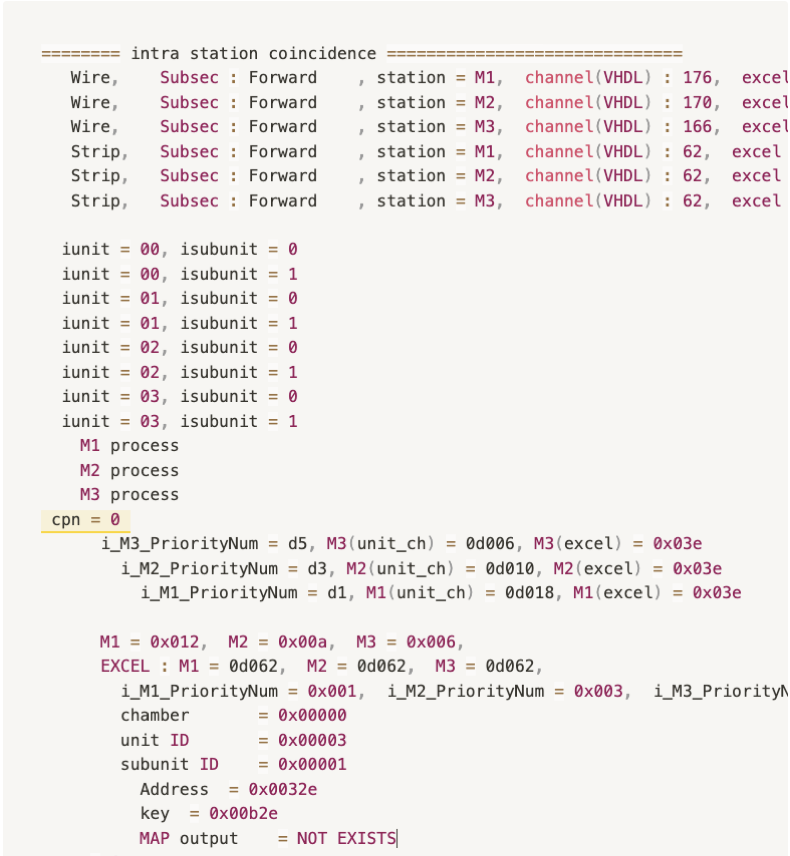
\includegraphics[width=16cm]{fig/Test/Bitwise_example.png}
  \caption[Strip Segment ReconstructionにおけるBitwiseシミュレーターのログ]{CStrip Segment ReconstructionにおけるBitwiseシミュレーターのログ}
  \label{Bitwise_example}
\end{figure}

このLUTのミスはソフトウェアシミュレーターで使われているrootファイル形式のものから、本番で使用するテキストファイル形式に整形する過程で生じたものである。そのため、ソフトウェアシミュレーターで検出することができず、本番とLUTを用いる実機試験で初めてわかった問題である。

\paragraph{Wire Segment Reconstruction}  
\par
Wire Segment Reconstructionではエンドキャップ領域の検出器の中心あたりで大きなInefficiencyが確認された。この不具合はスタッガードIDの割り振り方のミスによるものであると理解され、ケーブリングデータベースの修正が行われた。もともと、TGC検出器はステーションごとの$\eta$位置分解能が等しくなるように設計されており、設置によるずれが生じた後でも通し番号的にスタッガードIDを割り振れば同じ$\eta$をカバーするチャンネルを一意に定められると考えられていた。しかし、本実験の結果により、通し番号的にスタッガードIDを割り振ると、検出器の中央あたりの領域で$\eta$位置にずれが生じることが明らかになった。図\ref{Stag300}に通し番号的にスタッガードIDを振った時の各ステーションの$\eta$位置を示す。左にコインシデンスを取ることができたスタッガードID 100 ~ 105までの点を、右にコインシデンスを取ることができなかったスタッガーID 300 ~ 305の$\eta$位置を示す。通し番号的にスタッガードIDを振ると$\eta$が1.5 あたりの領域でステーションごとの$\eta$位置にずれが生じることがわかる。

\begin{figure}
\begin{minipage}[b]{.5\linewidth}
\centering
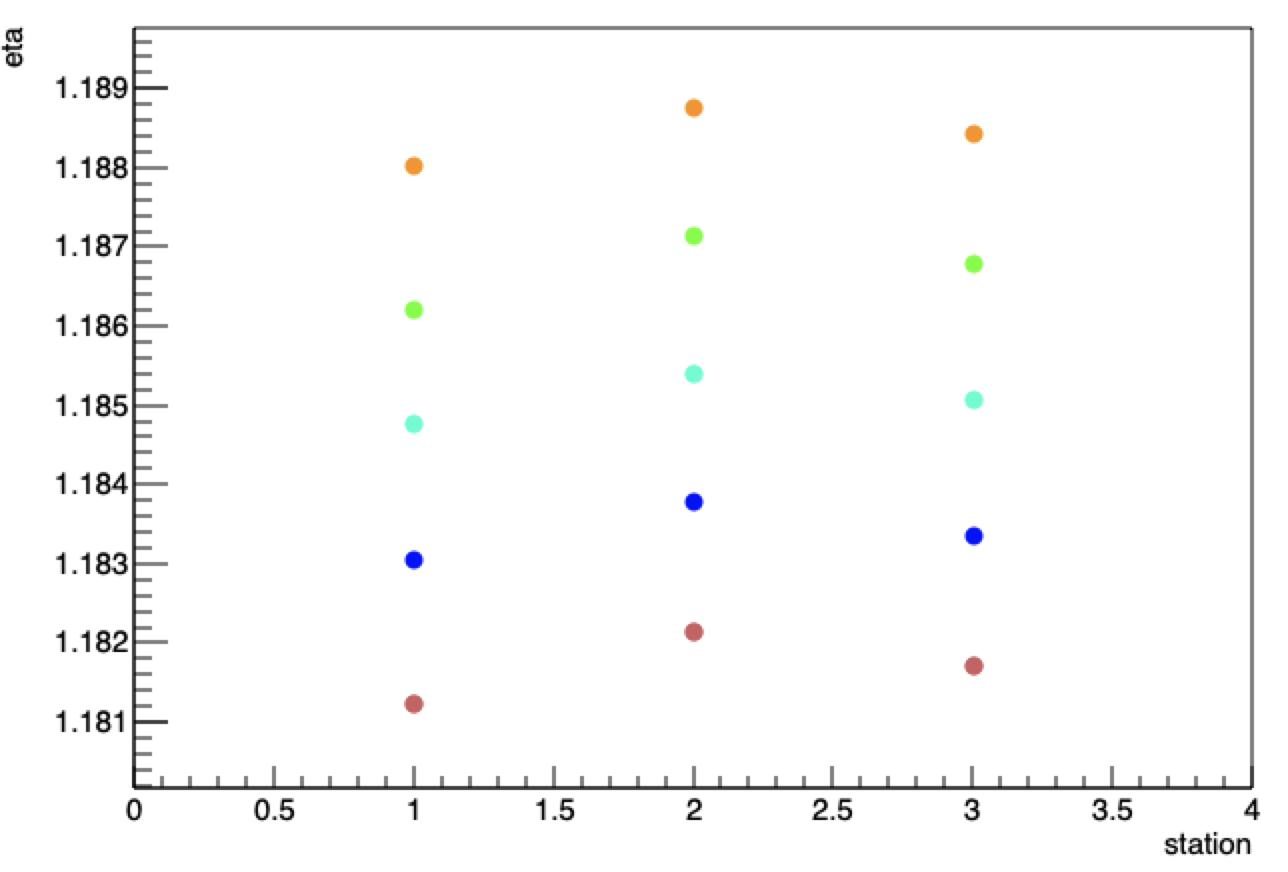
\includegraphics[height=5cm]{fig/Test/Stag100-105.png}
\subcaption{(a)}
\end{minipage}%
\begin{minipage}[b]{.5\linewidth}
\centering
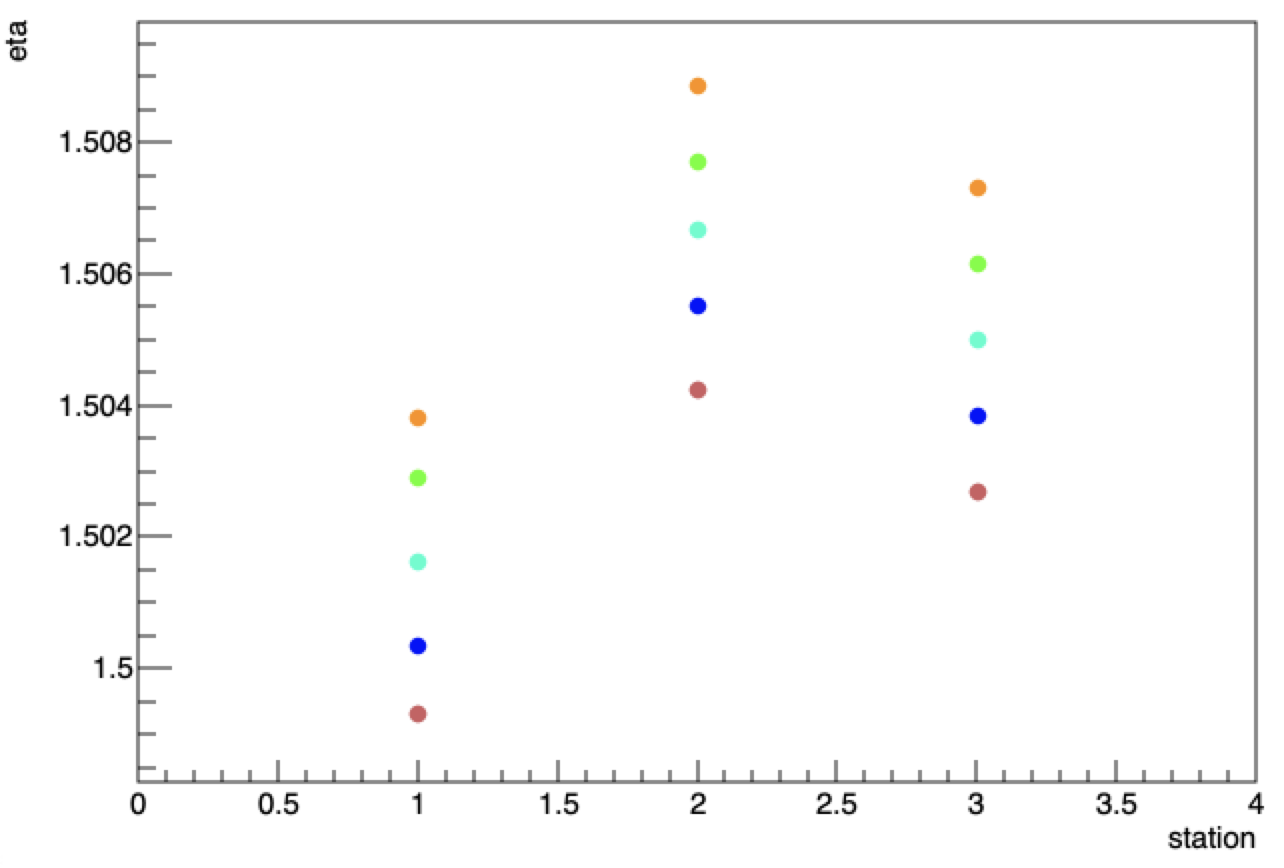
\includegraphics[height=5cm]{fig/Test/Stag300-305.png}
\subcaption{(a)}
\end{minipage}%
\caption[Wireでのスタッガードチャンネルのずれ]{Wireでのスタッガードチャンネルのずれ}
\label{Stag300}
\end{figure}

\paragraph{Wire Strip Coincidence}  
\par
Wire Strip CoincidenceではStrip、WireそれぞれのInefficiencyに加えて、未だ解決されていないWire スタッガードID 400 番以降の不具合が見えている。